\section{Introduction}
Thermal Control Systems of satellites are one of the major subsystems that contribute and sustain the life of a spacecraft. Thus, this lab is focusing on the application of various techniques in order to analyse first a simple geometric figure and then a more complex structure, the SPOT satellite. In general, the most crucial phases during a mission occur during the beginning and the end of the spacecraft lifetime, further denoted as EOL respectively BOL, and during the Hot and the Cold Case of the orbit.\\
To analyse these critical time frames, a Software developed by Airbus Defence \& Space, SYSTEMA, is used. SYSTEMA is a framework of different software packages, which include Thermica and Thermisol. These will be used in the further report to model, calculate and analyse the aforementioned geometric figures. \\In particular, the software breaks the analysis down into two main parts: the analysis of radiative phenomena during the orbits of the spacecraft and a nodal analysis based on a thermal equilibrium.

\section{Rejection Capacity Calculation}
\subsection{Geometric Model of a Cube in Thermica}
The first step to a thermal analysis is the modelling of our geometric figure, since at first we will analyse radiating surfaces. As stated before, in this part only a simplified geometric model of the SPOT satellite is used to familiarise with and gain a basic understanding of Thermica/Thermisol.\\
These simplified surfaces are supposed to be coated with aluminised SSM with an emissivity of $\epsilon = 0.78$ and an absorptivity of 0.15 at BOL and 0.19 at EOL (5 years).
 
\subsection{Solar, planetary IR and Albedo Flux}
After having obtained a geometric model, the mission parameters have to be defined. In particular, these parameter contain the trajectory as well as the kinematics of the previously defined geometric shape.\\
To specify these parameters, Thermica offers the option to create a \textit{mission}, i.e. an orbit with specified parameters: orbit height of 830km, Sun-synchronous with the ascending node at 10:30 pm local time, the -Z axis of the cube pointing (always) towards the earth and -Y axis in direction of travel. Now the two worst cases (Hot and Cold) are analysed, where the Hot Case occurs during winter solstice (closer to the sun) and the Cold Case during summer solstice.\\
By running a simulation with these parameters, Thermica is able to generate appropriate values for the Solar and planetary (IR and Albedo) flux, see \cref{tab:hotcase_cube} and \cref{tab:coldcase_cube}.



\begin{table}[!htb]
    \caption*{Solar and Planetary Flux Values}
    \begin{minipage}{.5\linewidth}
    \centering
      \caption{Hot Case}
      \label{tab:hotcase_cube}
		\begin{tabular}{|c | c | c | c|}
			\hline
			Surface & $Q_{sol}$ & $Q_{alb}$ & $Q_{IR}$ \\
			\hline
			$-Y_s$ & 59.00 & 5.90 & 36.00\\ \hline
			$+X_s$ & 72.00 & 6.40 & 36.00\\ \hline
			$+Y_s$ & 59.00 & 5.90 & 36.00\\ \hline
			$-X_s$ & 0.00 & 5.30 & 36.00\\ \hline
			$+Z_s$ & 79.00 & 0.00 & 0.00\\ \hline
			$-Z_s$ & 11.00 & 21.00 & 131.00\\ \hline
		\end{tabular}
    \end{minipage}%
    \begin{minipage}{.5\linewidth}
      \centering
        \caption{Cold Case}
        \label{tab:coldcase_cube}
		\begin{tabular}{|c | c | c | c|}
			\hline
			Surface & $Q_{sol}$ & $Q_{alb}$ & $Q_{IR}$ \\
			\hline
			$-Y_s$ & 45.00 & 4.50 & 36.00\\ \hline
			$+X_s$ & 39.00 & 4.80 & 36.00\\ \hline
			$+Y_s$ & 45.00 & 4.50 & 36.00\\ \hline
			$-X_s$ & 0.00 & 4.20 & 36.00\\ \hline
			$+Z_s$ & 61.00 & 0.00 & 0.00\\ \hline
			$-Z_s$ & 8.00 & 16.00 & 131.00\\ \hline
		\end{tabular}
    \end{minipage} 
\end{table}

Thermica also allows to plot different incident fluxes during a specified time, e.g. one orbit. Some of these plots are given in \cref{fig:coldcase_sol,fig:hotcase_sol,fig:coldcase_alb,fig:hotcase_alb}.
These graphs give a very detailed overview of how the incoming flux evolves for each side of the cube, this can be seen very easily in e.g. \cref{fig:hotcase_alb}, the Albedo Flux in the Hot Case, where the Flux is very high when the sun is directly behind the satellite, thus the reflected part is very high at this point.



\begin{figure}[h!]
\centering
  \centering
  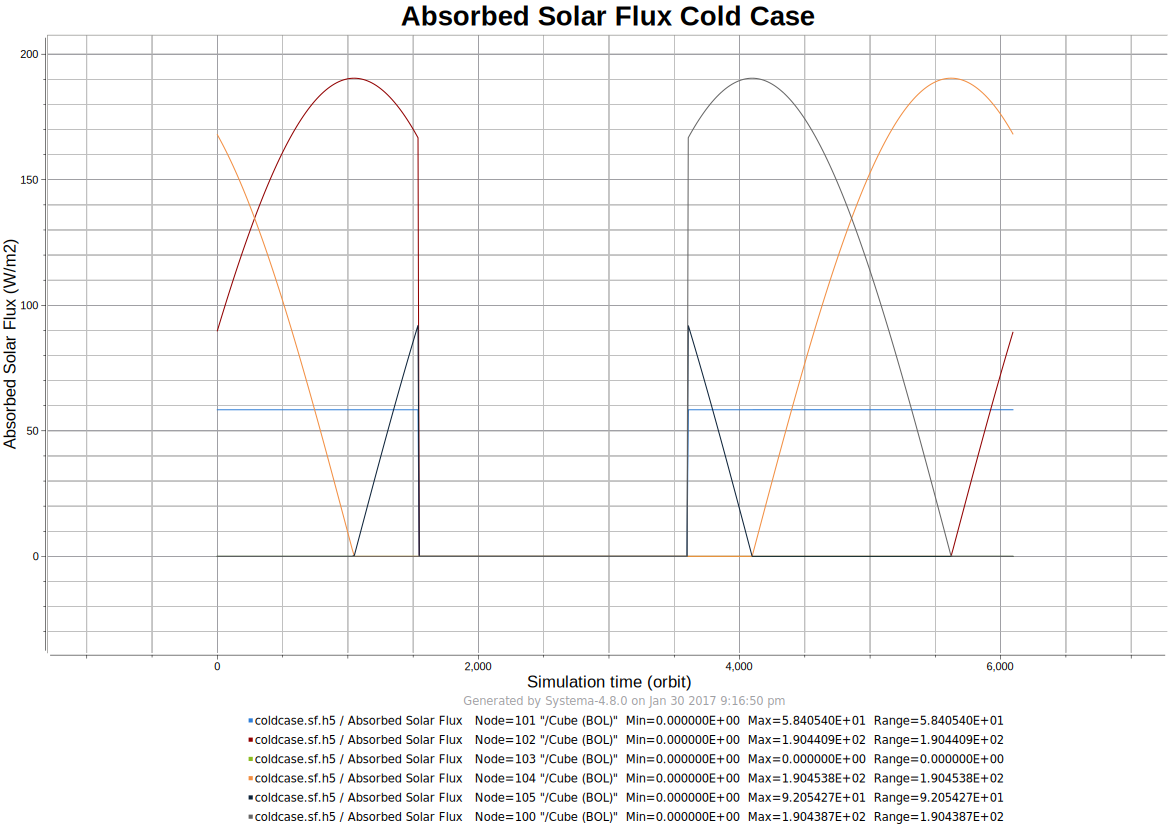
\includegraphics[width=0.7\linewidth]{images/Solar_flux_coldcase_BOL}
  \captionof{figure}{Cold Case Solar Flux}
  \label{fig:coldcase_sol}
\end{figure}
\begin{figure}[h!]
  \centering
  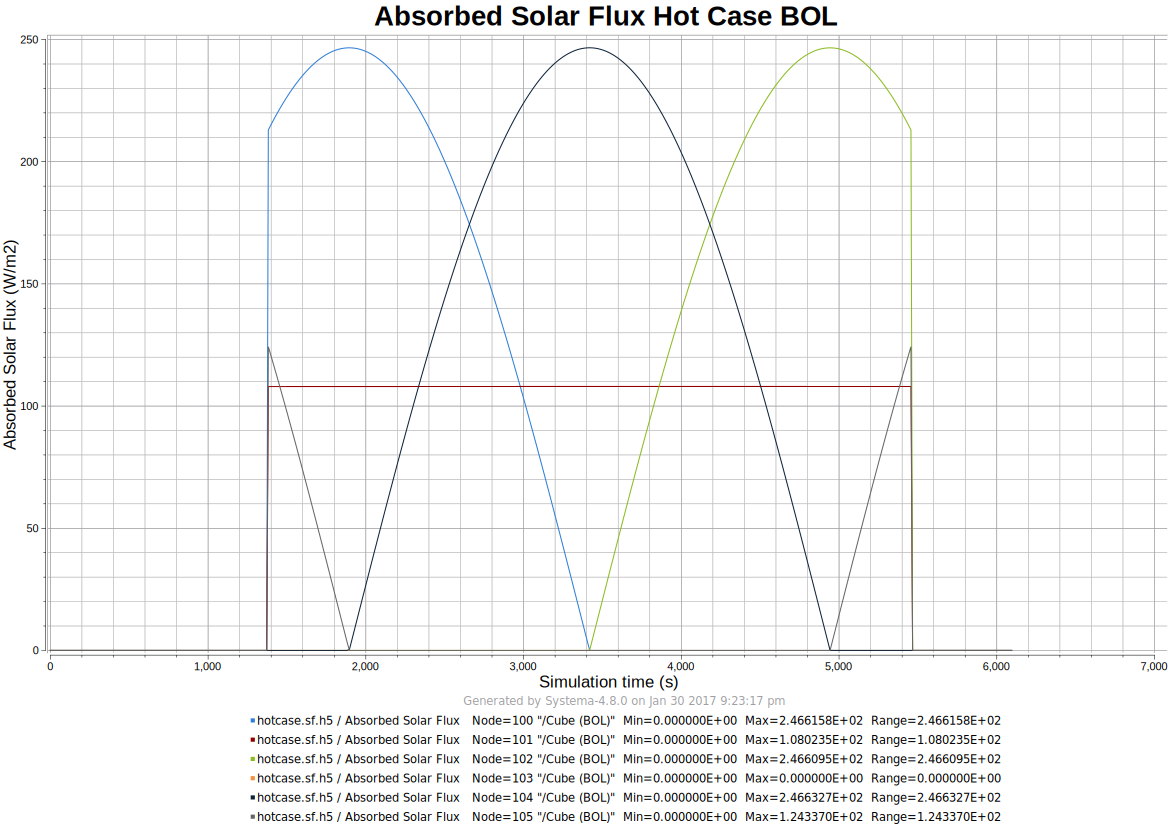
\includegraphics[width=0.7\linewidth]{images/Solar_flux_hotcase_BOL}
  \captionof{figure}{Hot Case Solar Flux}
  \label{fig:hotcase_sol}
\end{figure}

\begin{figure}[h!]
\centering
  \centering
  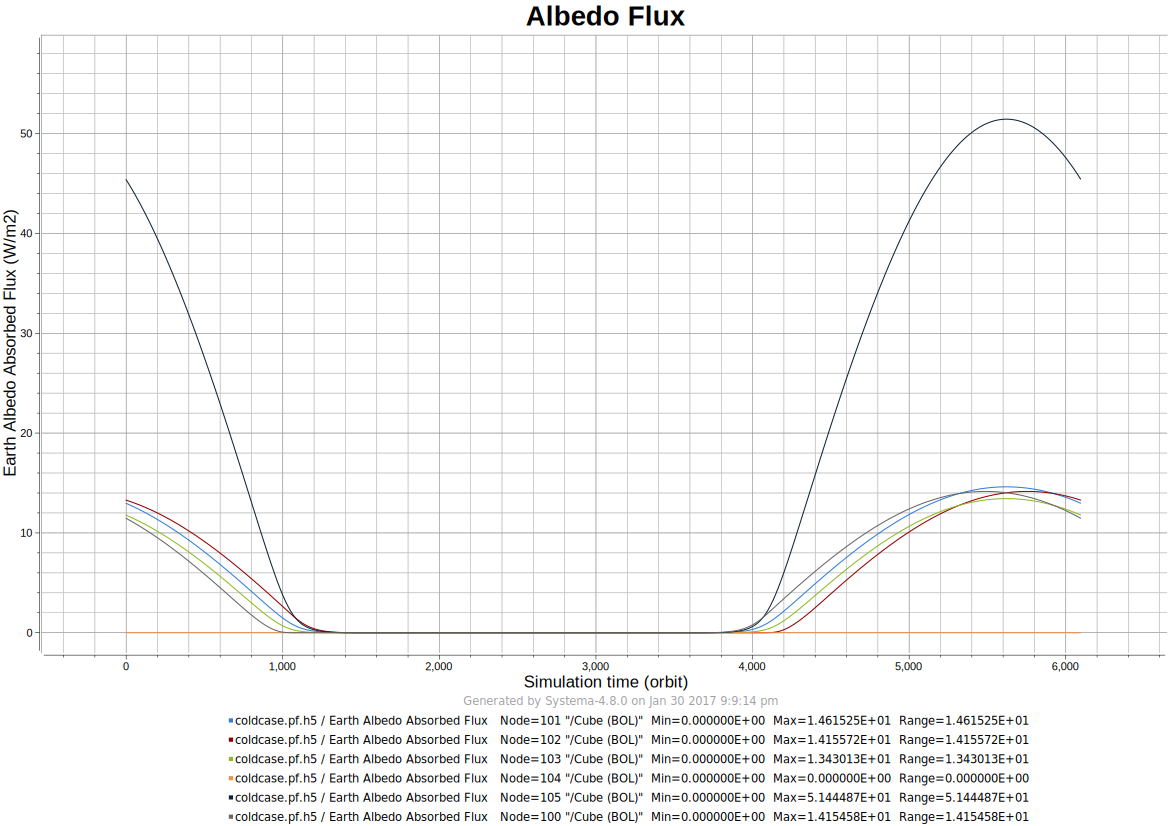
\includegraphics[width=0.7\linewidth]{images/albedo_flux_coldCase_BOL}
  \captionof{figure}{Cold Case Planet Albedo Flux}
  \label{fig:coldcase_alb}
\end{figure}
\begin{figure}[h!]
  \centering
  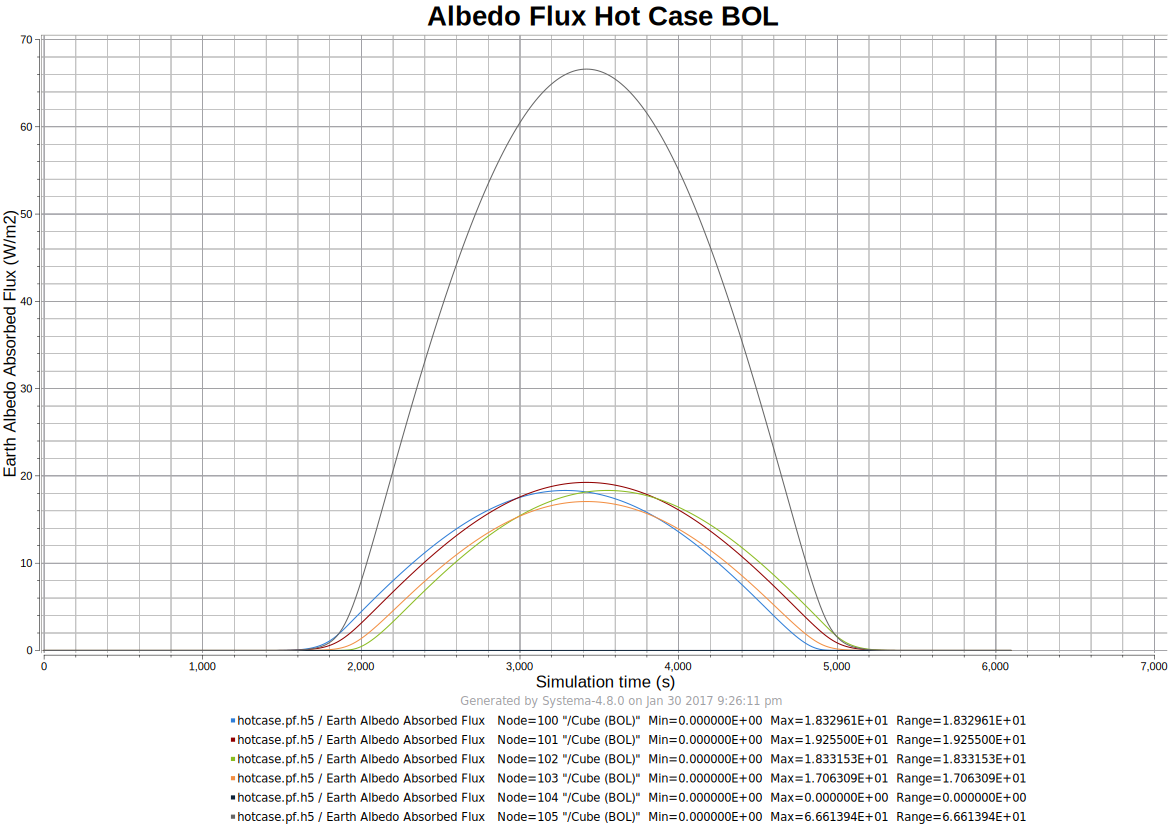
\includegraphics[width=0.7\linewidth]{images/albedo_flux_hotcase_BOL}
  \captionof{figure}{Hot Case Planet Albedo Flux}
  \label{fig:hotcase_alb}
\end{figure}

\newpage

\subsection{Rejection Capacity}
Having obtained the absorbed flux values for each side of the cube, we can now calculate the rejection capability of the aluminised SSM. For the End-of-Life, at winter solstice, an average temperature of 35°C is assumed and for the Beginning-of-Life, at summer solstice, an average temperature of 0°C.\\
The calculation was then done according to the following equation:
\begin{equation}
\centering
	R_c = \epsilon \sigma A T_{avg}^4 - Q_{sol} - Q_{alb} - Q_{IR}
	\label{eq:rejcap}
\end{equation}

Applying \cref{eq:rejcap}, we can obtain the following values for the rejection capacities for each side of the cube:

\begin{table}[!htb]
    \caption*{Rejection Capacities for each cube surface}
    \begin{minipage}{.5\linewidth}
    \centering
      \caption{Hot Case}
      \label{tab:hotcase_rejcap}
		\begin{tabular}{|c | c |}
			\hline
			Surface & Rejection capacity $\frac{W}{m^2}$ \\
			\hline
			$-Y_s$ & 303.60  \\ \hline
			$+X_s$ & 290.10 \\ \hline
			$+Y_s$ & 303.60 \\ \hline
			$-X_s$ & 363.20 \\ \hline
			$+Z_s$ & 325.50 \\ \hline
			$-Z_s$ & 241.50 \\ \hline
		\end{tabular}
    \end{minipage}%
    \begin{minipage}{.5\linewidth}
      \centering
        \caption{Cold Case}
        \label{tab:coldcase_rejcap}
		\begin{tabular}{|c | c |}
			\hline
			Surface &  Rejection capacity $\frac{W}{m^2}$ \\
			\hline
			$-Y_s$ & 160.16 \\ \hline
			$+X_s$ & 165.86\\ \hline
			$+Y_s$ & 160.16 \\ \hline
			$-X_s$ & 205.46 \\ \hline
			$+Z_s$ & 184.66 \\ \hline
			$-Z_s$ & 90.66 \\ \hline
		\end{tabular}
    \end{minipage} 
\end{table}

In the Hot Case the radiative contribution was calculated with $T_{avg} = 36.25 ^{\circ} C$, thus leading to a radiative contribution of $T_{avg} = 404.50 K$.

\section{Thermal Dimensioning of SPOT Satellite Platform}

After having investigated the corresponding fluxes for the applied orbit in the two different cases, as well as the rejection capacities for each side of a cube satellite, we use these results to determine the thermal distribution inside the satellite platform of SPOT. For this, we extend the cube model used before by assuming that it contains 4 different equipments inside, as well as 4 radiators outside for each equipment. The remaining 2 sides of the cube will have no radiators, since we assume that the batteries and the payload are connected to those sides. Within Thermica, we start by using the geometric models for the cold case, SPOT-BOL, and end of life, SPOT-EOL. 

\subsection{Positioning of the equipment}
The very first important step of the analysis is to determine the best places to put the equipment, i.e. on which side of the cube depending on the equipment's specification and the fluxes calculated before. These specifications are listed in table \ref{tab:equipmentspecification}

\begin{table}[h!]
\centering
\begin{tabular}{ | c| c|c|c|c|c|c|c| }
\hline 
&  \multicolumn{2}{|c|}{Nominal Mode} &  \multicolumn{2}{|c|}{Safe Mode} & & \multicolumn{2}{|c|}{Dissipated Power [W] }\\
Function & Tmin & Tmax & Tmin & Tmax & Mass & nominal mode & safe mode  \\
& \multicolumn{2}{|c|}{$^{\circ}$C} & \multicolumn{2}{|c|}{$^{\circ}$C} & kg &Operation/Stand-By &  \\  \hline

Power Supply &-10   & 40  & -15&50  & 40  &  150 /50 & 20  \\ \hline
On-board Computer &-10  & 40 &-15 &50 &5 &15 /10& 10 \\ \hline
Attitude Control &-10  &40 & -15& 50&30 &110/50 &30  \\ \hline
Telemetry &-10  &40 &-15 &50 &20 &70/0 & 0  \\ \hline
\end{tabular}
\caption{Specifications for equipments}
\label{tab:equipmentspecification}
\end{table}

To place the equipment in the most efficient way, we exclude the $X$-axis, since the batteries, solar panels and the payload are going to be placed there. For the arrangement, we consider the rejection capacities of each of the sides in the hot case scenario and power consumptions of the equipments. Also, one has to consider the safe mode, which provides basic functions of the satellite by pointing the +$Z_{s}$ side towards the sun, which results in a strong solar flux. The resulting best arrangement is listed in table \ref{tab:arrangement}

\begin{table}[H]
\centering
\begin{tabular}{ | c| c|}
\hline 
Side & Equipment  \\ \hline
$-Y_{s}$ & Power Supply  \\ \hline
$-Z_{s}$ &On-board Computer \\\hline
$+Y_{s}$ &Attitude Control \\ \hline
$+Z_{s}$ &Telemetry   \\ \hline
\end{tabular}
\caption{Chosen arrangement of equipment}
\label{tab:arrangement}
\end{table}
From this arrangement, we can relate the rejection capacities of the individual sides to the corresponding equipment. Also, we calculated the heat capacities of each equipment by multiplying the mass with the specific heat capacitance of $900\frac{\mathrm{K}}{\mathrm{kgK}}$.


\begin{table}[H]
\centering
\begin{tabular}{ | c| c|c|c|c|}
\hline 
Side & Equipment  & Rejection Capacity [$\frac{\mathrm{W}}{\mathrm{m}^{2}} $] & \specialcell{Mass of \\Equipment [kg]} & Thermal Capacity [$\frac{\mathrm{K}}{\mathrm{K}}$]   \\ \hline
$-Y_{s}$ & Power Supply & 303.6 & 40 &  36000   \\ \hline
$-Z_{s}$ &On-board Computer&  242.5 & 5 & 4500 \\\hline
$+Y_{s}$ &Attitude Control  &  303.6 & 20& 18000 \\ \hline
$+Z_{s}$ &Telemetry & 325.5 & 20 &  18000 \\ \hline
\end{tabular}
\caption{Equipment with heat capacities and rejection capacities.}
\label{tab:arrangement}
\end{table} 

\subsection{Sizing of Radiators}
Once  the positions of the equipment are defined, we are able to size the radiators according to the power consumptions and heat capacities. The required area can be calculated using $A=\frac{P_{diss}}{Q_{s,i}}$, where $Q_{s}$ are the rejection capacities for the individual sides at the hot case and $P_{diss}$ the power that is dissipated by the equipment.


\begin{table}[H]
\centering
\begin{tabular}{ | c| c| c| }
\hline 
Side & Equipment  & Areas [$m^{2}$] \\ \hline
$-Y_{s}$ & Power Supply & 0.49   \\ \hline
$-Z_{s}$ &On-board Computer & 0.06   \\\hline
$+Y_{s}$ &Attitude Control &  0.36 \\ \hline
$+Z_{s}$ &Telemetry  &    0.22 \\ \hline
\end{tabular}
\caption{Required radiator sizes in the hot case}
\label{tab:arrangement}
\end{table}

 
\subsection{Dimensioning of Heating Power}
After the sizing of the radiator areas is performed using the hot case, the additional heating power, that might be required in the cold case, has to be determined. For that, we calculate the power that is actually evacuated in the cold case using the heat capacities in the cold case and the radiator sizes calculated before. From that, we reduce the power that is dissipated by the equipment in the hot case as listed in table \ref{tab:equipmentspecification}. This difference is the power that is lost and results in a continuous cooling, so this difference in power has to be added by heating to avoid further cooling. We assume that the additional heating power avoids the equipment to drop below $-5^{\circ}$C, as defined in the cold case of the cube before Table lists the calculated evacuated power in this case, as well as the dissipated power in the hot case for each equipment and and the resulting required heating:


\begin{table}[H]
\centering
\begin{tabular}{ | c| c| c| c|c|}
\hline 
Direction& Equipment  & \specialcell{Evacuated \\ Power [W]} & \specialcell{Dissipated\\Power [W]} & \specialcell{Heating \\ Power [W]} \\ \hline
$-Y_{s}$ & Power Supply &  50 & 79 & 29    \\ \hline
$-Z_{s}$ &On-board Computer &10 &6 &  0  \\\hline
$+Y_{s}$ &Attitude Control & 50 & 58 & 8  \\ \hline
$+Z_{s}$ &Telemetry  &  0   & 40 & 40 \\ \hline
\end{tabular}
\caption{Power calculations in cold case}
\label{tab:arrangement}
\end{table}

\section{Thermal Calculations for SPOT}
In order to test and verify our previous calculations, we simulate the thermal behaviour of our SPOT satellite using Thermica to proof that the satellite fulfils the requirements of staying within $-5^{\circ}$ and $40^{\circ}$. We used the geometric models in the hot case and in the cold case for the satellite SPOT4,  which were already provided. Since we have more information now about the satellites compared to the first simplified cube simulations, we also have to adapt several files throughout the simulation. 

\subsection{Nodal network}
In thermica, interactions are described using the so called nodal network, where as an example the output of several simulation elements is linked to further simulation elements that need that data is input. Therefore, the nodal network gives an overview about the interactions of different simulation elements. In our case, the different equipments are assigned different node numbers, i.e. 3 to the $+Y_{s}$ side of the cube and thus to the attitude control, 4 to the power supply side,  5 to the telemetry side and 6 to on-board computer. The $\pm X$ sides are left out since they are not considered in this thermal simulation as they are connected to the batteries and payload.

\subsection{Radiative Phenomenon}
In the thermal simulation we consider the hot and the cold case, end of life and beginning of life. For setting up the simulation, several elements defining the mission, which depends on the case, the nodal description, "Radiation", "Solar fluxes", "Planetary fluxes, "Skeleton" and finally "Solver" have to be connected within Thermica. However, we need to adapt several files before using the latter two elements in the simulation, so these are deactivated for the first run of the simulation.  
The reason for that extra step is that the created file called "Spot.usr.nwk", which contains information about the radiative interactions of the several elements, assumes e.g. a radiator surface area of $1$ m$^{2}$ and other different values. However, to adapt the simulation to our case, we have to change these values in the file. In order to do so, one has to add the various values calculated above like the different fluxes for each radiator, heat capacities and dissipations. Once these changes are done, one can run the simulation with the last steps including the Thermica solver THERMOSOL.

\section{Results}
The results are shown in the figure \ref{fig:spothot} and describing the temperature for every node, i.e. side of the cube of SPOT, during the simulation for about 20 orbits. As one can see in the hot case, it is verified that the previous calculations of the radiator sizes avoid a heating above 40 degrees, since the temperatures converge towards that value over time. 
\begin{figure}[H]
	\centering
	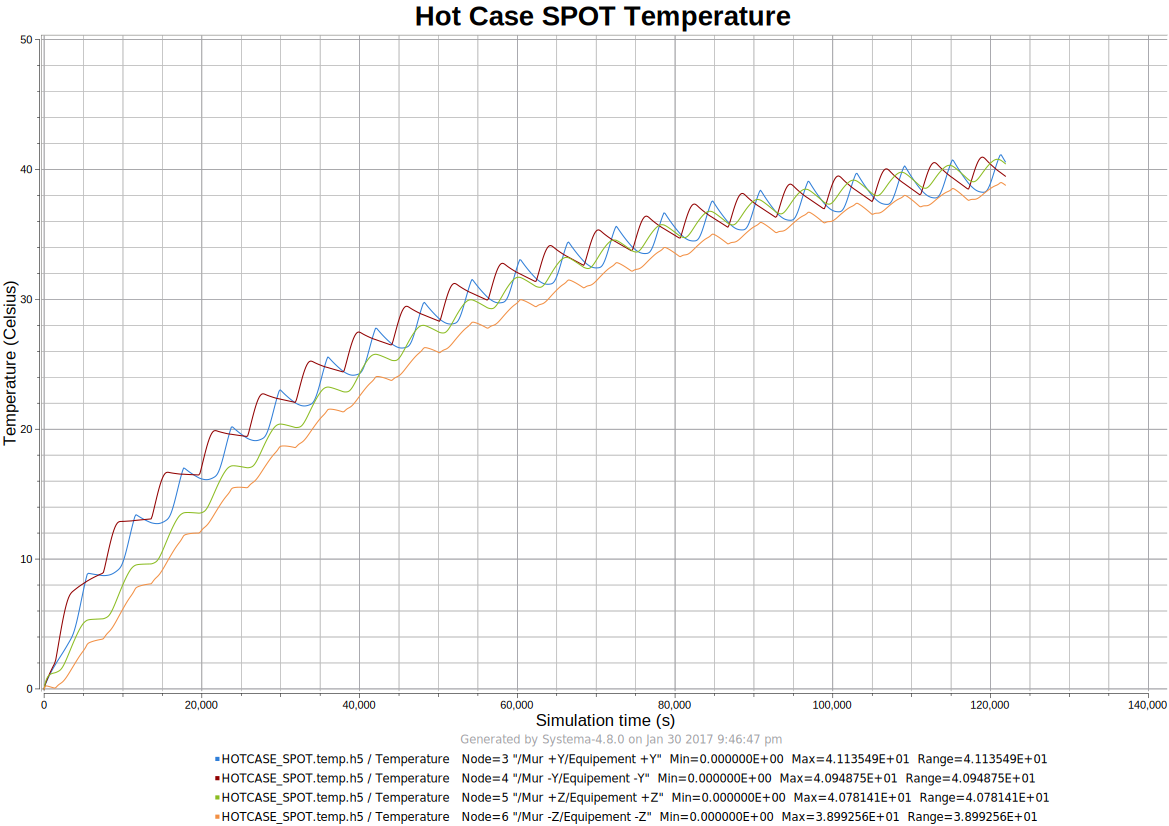
\includegraphics[scale=0.15]{images/SPOT_hotcase_temperature.png}
	\caption{Temperature of SPOT nodes in the hot case}
	\label{fig:spothot}
\end{figure}

\begin{figure}[H]
	\centering
	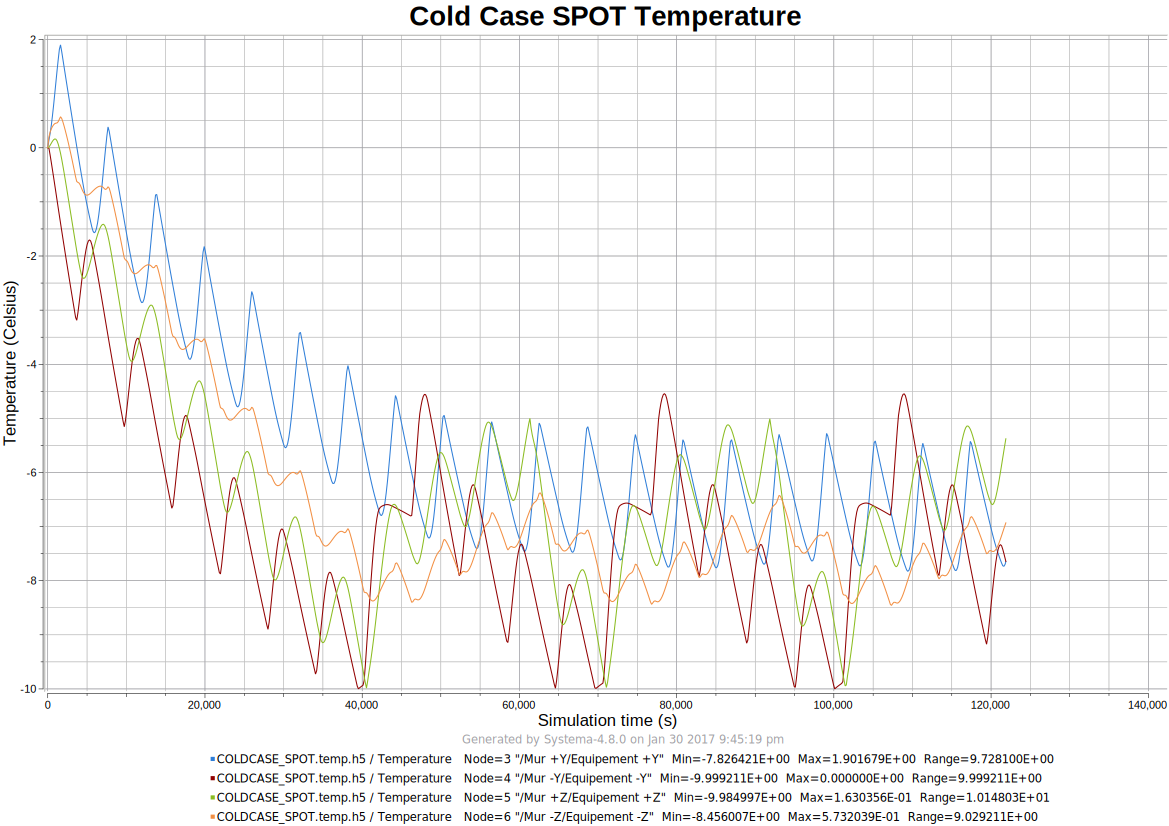
\includegraphics[scale=0.15]{images/SPOT_coldcase_temperature.png}
	\caption{Temperature of SPOT nodes in the cold case}
	\label{fig:spothot}
\end{figure}


Also in the cold case, one can see of the systems is heated up as soon as it gets close to $-10^{\circ}$, and therefore further cooling is avoided.

\section{Conclusion}
In this report, we simulated the thermal behaviour of a simple satellite using Thermica. In a first step, a simple cube was simulated in the hot case and cold case, or end of life and beginning of life. The different fluxes resulting from the Sun, Earth's albedo and the Infrared radiation from Earth were simulated for each side of the cube. Also, we calculated the heat rejection capacities of the cube for the two cases, hot and cold.
In the second step of the simulation, we used these result to further simulate the thermal behaviour inside the satellite SPOT. In a first step, an optimised arrangement of several equipment elements was performed. In addition, the radiator sizes for each side of the satellite were calculated in order to prevent the equipment from overheating, while also the required heating power in the cold case resulting from that was obtained for each of the equipment. In a final simulation, it was verified that the specific requirements, i.e. the temperature range, is met by the chosen values for the radiator sizes and heating power. The whole simulation provided us a very interesting introduction into the use of Thermica and the way thermal analysis is performed.
